\begin{figure}[tbp]
    \centering
    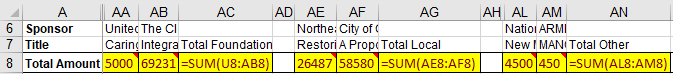
\includegraphics[width=\columnwidth]{figure/figure3.png}
    \caption{用于展现\wa 的多个单元格有效性精化方法的工作表``Detail for the College of A\&S''。\cu 检测出一个单元格类(用黄色标记),并进而导致六个假阳性的缺陷被报告出来(用红色三角形标注),不过这六个单元格会被\wa 的多单元格有效性精化方法从类中排除出去,进而不会再被错误的标记为有缺陷的单元格。}
    \label{figure3}
\end{figure}